\documentclass[12pt]{article}
% Margin fixes
\oddsidemargin -0.5in
\evensidemargin -0.5in
\textwidth 7.25in
\topmargin 0.0in

\headheight 0.0pt
\headsep 0.0pt
\voffset 0.0pt
\textheight = 9.0in
\usepackage{amsmath,amssymb,graphicx,float}

\title{Absorption of Radiation}
\author{Nathan Grouse\\Lisa Tran}

\newcommand{\counts}{\text{ counts}}

% Start the document!
\newcommand{\documentname}{\textsl{Article}}
\begin{document}
\maketitle

\section{Introduction}
\indent \indent The purpose is to observe how different materials absorb $\beta$ and $\gamma$ radiation.

\subsection{Apparatus}
\indent \indent The apparatus includes a Geiger-Muller Counter, a source of $\beta$ radiation, and a source of $\gamma$ radiation. The Geiger-Muller tube consists of a wire inside of a cylinder that contains a gas at low pressure. When radiation enters the tube and ionizes some of the gas inside, liberated electrons accelerate towards the wire, which is kept at a high voltage relative to the metal walls of the tube. As these electrons are accelerated they ionize more of the gas and an electron avalanch ensues. The Geiger-Muller counter detects each of these pulses.

\begin{figure}[H]
\centering
\hspace{-0.0in}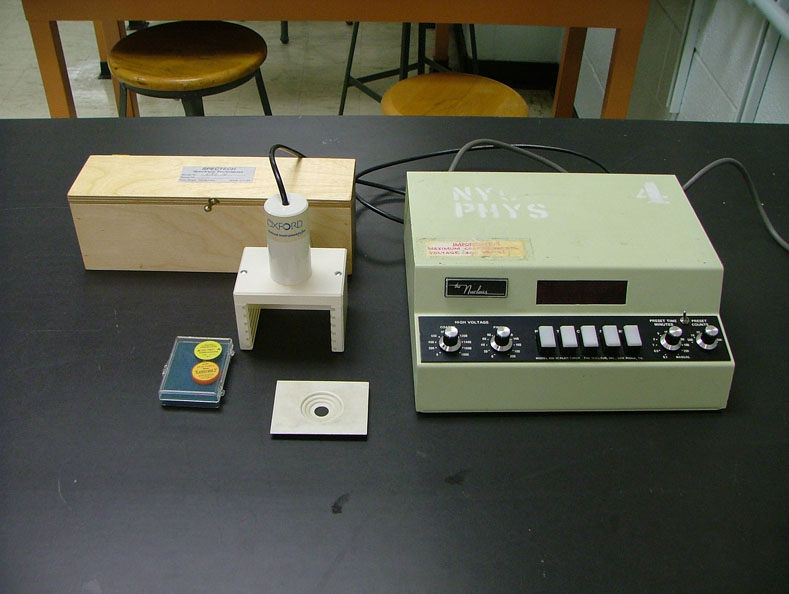
\includegraphics[scale=0.40]{apparatus.png}
\caption{Apparatus \label{fig:setup}}
\end{figure}

\section{Data}
\begin{figure}[H]
\centering
\hspace{-0.0in}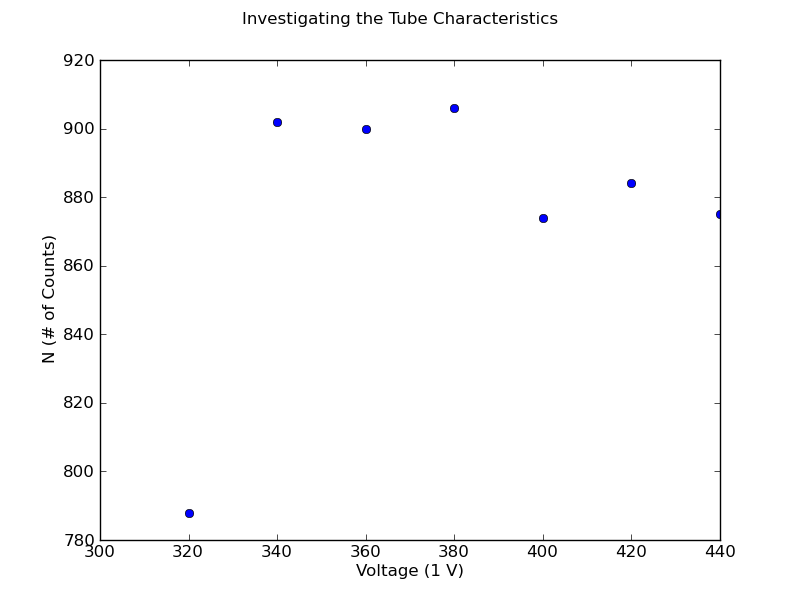
\includegraphics[scale=0.60]{Plot1.png}
\caption{Finding the plateau of the Geiger counter's counting rate \label{fig:setup}}
\end{figure}

\begin{figure}[H]
\centering
\hspace{-0.0in}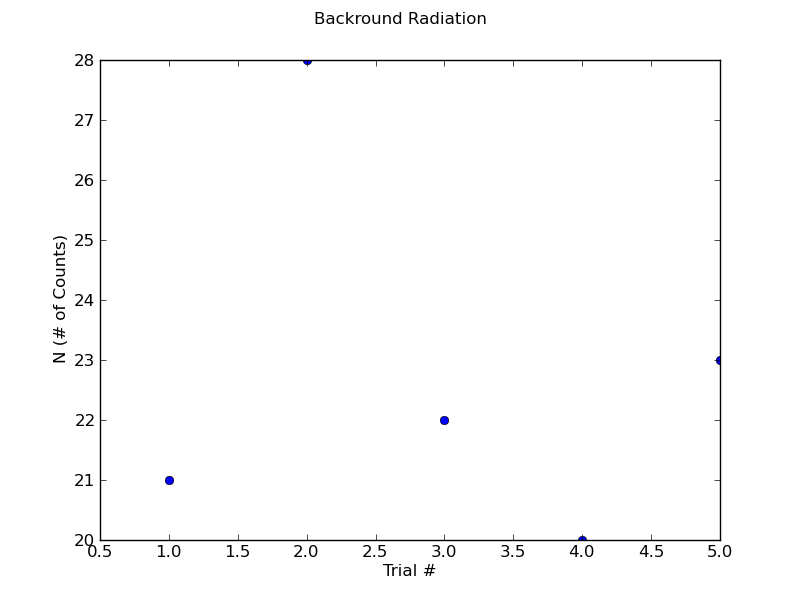
\includegraphics[scale=0.60]{Plot2.png}
\caption{Each trial counted backround radiation for 3 minutes \label{fig:setup}}
\end{figure}

\indent \indent Absorption of Beta Particles - after 1000 counts the timer stops. The timer marks $\frac{6}{10}$ second intervals.

\begin{figure}[H]
\centering
\hspace{-0.0in}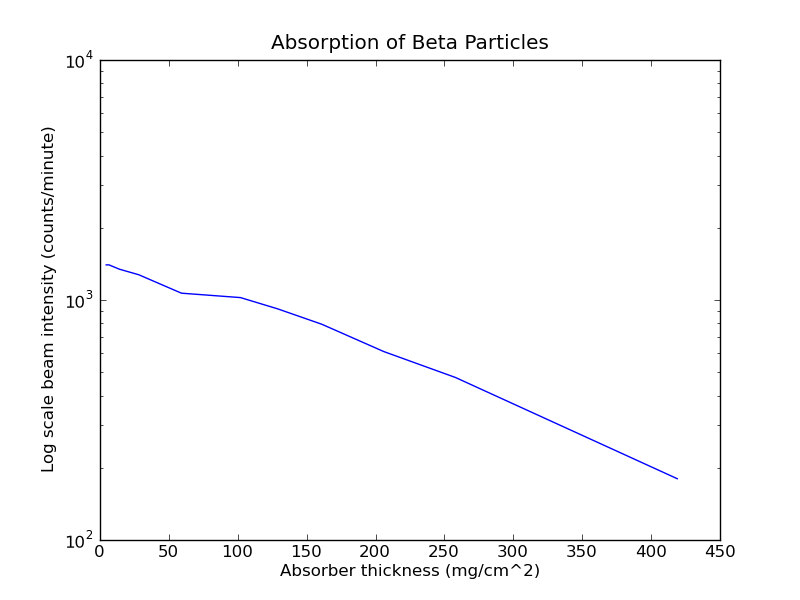
\includegraphics[scale=0.60]{Plot3.png}
\caption{The time interval was converted to minutes and inverted to find beam intensity in counts/minute. The average value for backround radiation (counts/minute) was subtracted from the beam intensity values. \label{fig:setup}}
\end{figure}

\indent \indent Absorption of Gamma Rays - after 500 counts the timer stops. The timer marks $\frac{6}{10}$ second intervals.

\begin{figure}[H]
\centering
\hspace{-0.0in}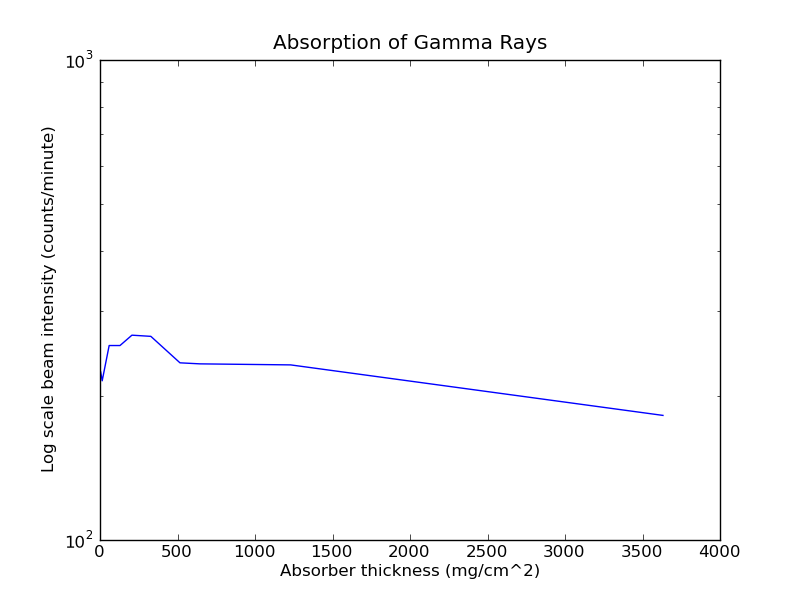
\includegraphics[scale=0.60]{Plot4.png}
\caption{Same process, but halfway through taking the data the fuse was changed. This made the data fit much better with expectations. This suggests that gamma rays have no trouble penetrating materials with thickness 1230 ($\frac{mg}{cm^2}$) or smaller. \label{fig:setup}}
\end{figure}

\section{Calculations}
\indent \indent Average Value of Backround Radiation Counts per Minute:
\[B_a_v_g = \frac{\frac{21+28+22+20+23}{5}}{3} \frac{counts}{minute} = 7.6 \frac{counts}{minute} \]

\section{Error Analysis}
\indent \indent Uncertainty in counts from a Geiger Counter is generally given by:
\[ \sigma = \sqrt{N_a_v_g} \]
\indent \indent For the recorded backround radiation rates, the square roots of the five values should fall within the $\sqrt{N_a_v_g}$ for average backround radiation rate:
\[ N_a_v_g = 22.8 \counts \
\sqrt{N_a_v_g} = 4.8 \
\sqrt{N_1} = 4.6 \
\sqrt{N_2} = 5.3 \
\sqrt{N_3} = 4.7 \
\sqrt{N_4} = 4.5 \
\sqrt{N_5} = 4.8 \ \]
\indent \indent % Error:
\[E_1 = |\frac{4.6-4.8}{4.8}| = 4.2 \ \% \]
\[E_2 = |\frac{5.3-4.8}{4.8}| = 10.4 \ \% \]
\[E_3 = |\frac{4.7-4.8}{4.8}| = 2.1 \ \% \]
\[E_4 = |\frac{4.5-4.8}{4.8}| = 6.3 \ \% \]
\[E_5 = |\frac{4.8-4.8}{4.8}| = 0 \ % \]

\indent \indent In summary, backround radiation was accounted for and the fuse was fixed in time to salvage the $\gamma$ ray section of the experiment. Error was adequately minimized.

\section{Conclusion}
\indent \indent I obtained reasonable results and I saw what I expected to see. In summary, $\gamma$ rays are more penetrative than $\beta$ particles, and the counting rate was higher for the $\beta$ particles because it was a fresher source - the $\gamma$ source had undergone a few half lifes.

\section{Questions}
1. Should the label side be up or down, or does it not make a difference? \\
During the experiment, the label side should be down because it does make a difference. I'll assume there is some sort of absorbant material inbetween the labeled side and the source and that the other side does not have much absorbing material. \\

2. Roughly, the five values (backround radiation) of the three minutes readings should fall within the $sqrt{N}$ of N. Do They? \\
Yes, they do. \\

3. What absorber thickness is necessary to cut this beta radiation to 1/2 of its original values? \\
Initially, it takes 71 time intervals for the $\beta$ sources to make 1000 counts. At a thickness of 206 $\frac{mg}{cm^2}$ it takes 162 time intervals. This is about half of the original value, so the thickness required is somewhere between 161 and 206 $\frac{mg}{cm^2}$ \\

4. Why do you think that nuclear physicists prefer $mg/cm^2$ as the unit for quoting results, instead of a simple linear dimension? \\
Probably because the surface or volume density of a material will help a nuclear physicist predict how easily radiation will penetrate a material much more accurately than a linear thickness. \\

5. Is your data points lie on a straight line, the beam attenuation is exponential with absorber thickness. Is it? \\
Yes, it is for both the $\beta$ and $\gamma$ plots. On the $\gamma$ plot this starts after the fuse was replaced. \\

6. Devise an experiment to check the square-root rule which is discussed in section 3.2 and 11.2 of "Error Analysis" by John Taylor. \\
The square root rule states that the uncertainty in any counted number of random events, as an estimate of the true average number, is the square root of the counted number. To check this assertion, set up a radiation source under a geiger counter and observe the number of counts for a fixed period. If the number of counts is x, speculate that if someone else were to perform this experiment with the same equipment just used, the number of counts that person would record would be within the range $x\pm \sqrt{x}$.

\end{document}